\subsection{Augmentation du $\alpha$ initial}

\subsubsection{Configuration, modifications et résultats attendus}

Grâce à l'étude préliminaire de notre implémentation de SAC sur 400
trajectoires, nous pouvons approximer un $\alpha$ pseudo-optimal qui a permis
d'atteindre les meilleurs scores. En effet, c'est quand $\alpha \approx 0.02$
que le score est maximale. Nous décidons d'initialiser cette valeur à $0.02$ dès
le départ. Nous attendons que chaque répétiton de l'apprentissage atteigne des
politiques optimales même après seulement 400 épisodes. L'étude est toujours répétée $10$ fois.

\subsubsection{Analyse}

\begin{figure}[H]
    \centering
    \begin{subfigure}{0.3\textwidth}
        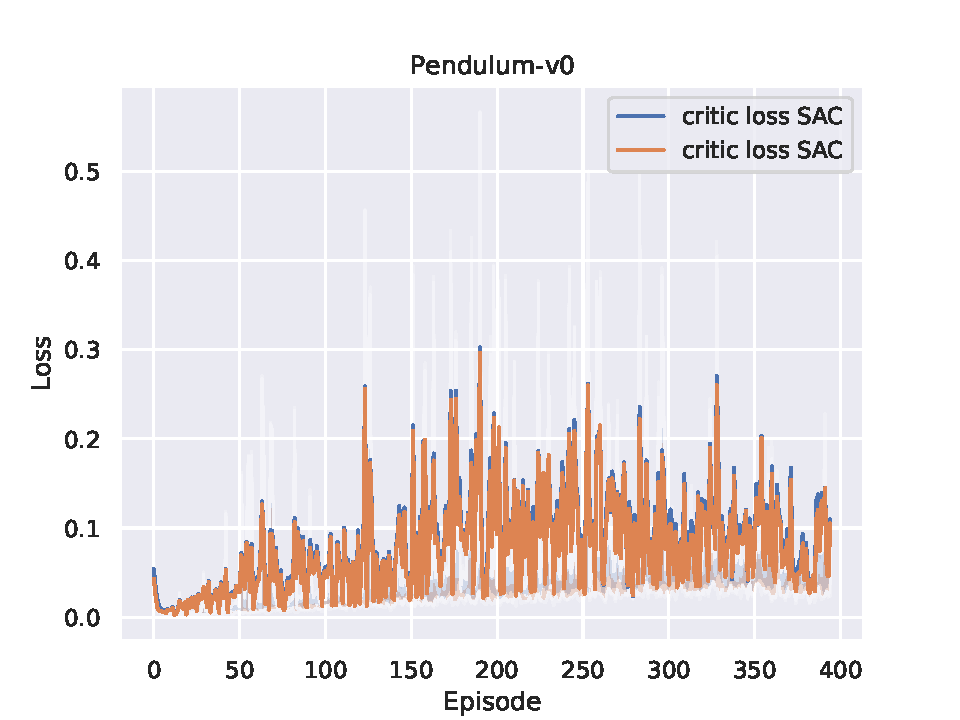
\includegraphics[width=\textwidth]{figures/sac_itr2/critic_loss_Pendulum-v0_pg_dataset_td_eval_True_cycles_40_trajs_20_batches_20_gamma_0.99_nstep_5_lr_act_0.01_lr_critic_0.01pg.pdf}
        \caption{Fonction de perte de la critique}
    \end{subfigure}
    \begin{subfigure}{0.3\textwidth}
        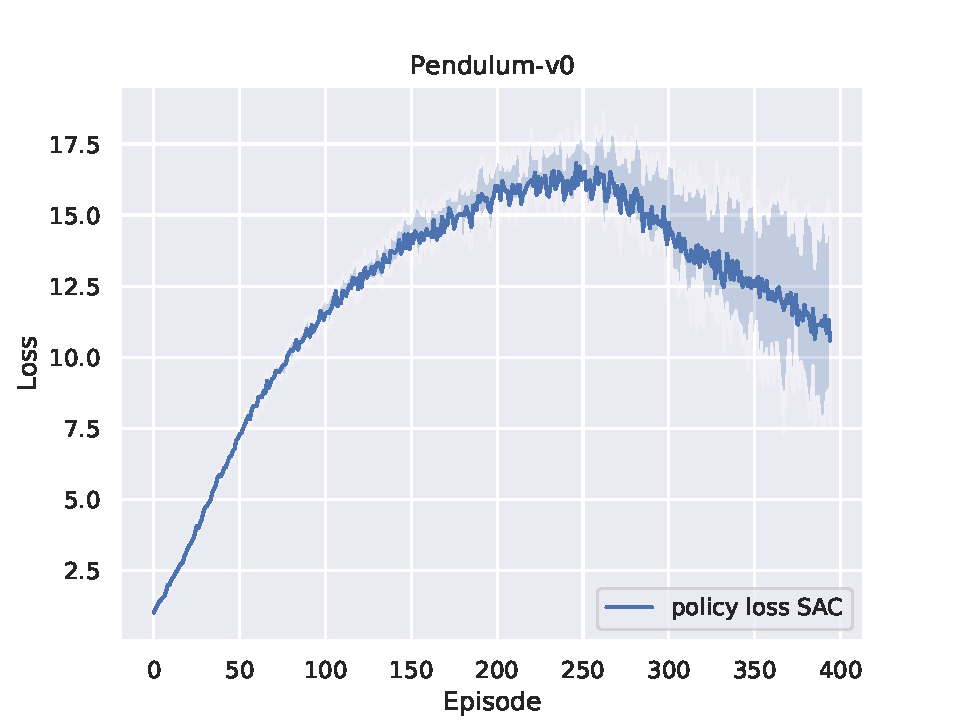
\includegraphics[width=\textwidth]{figures/sac_itr2/policy_loss_Pendulum-v0_pg_dataset_td_eval_True_cycles_40_trajs_20_batches_20_gamma_0.99_nstep_5_lr_act_0.01_lr_critic_0.01pg.pdf}
        \caption{Fonction de perte de la politique}
    \end{subfigure}
    \begin{subfigure}{0.3\textwidth}
        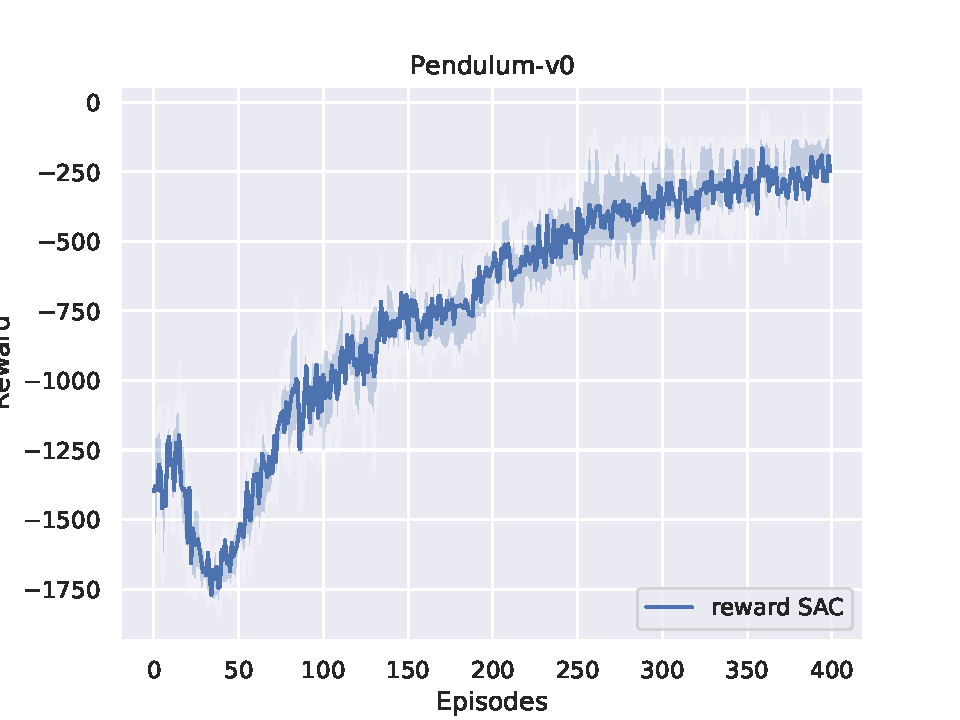
\includegraphics[width=\textwidth]{figures/sac_itr2/rewards_Pendulum-v0_pg_dataset_td_eval_True_cycles_40_trajs_20_batches_20_gamma_0.99_nstep_5_lr_act_0.01_lr_critic_0.01.pdf}
        \caption{Récompenses des épisodes}
    \end{subfigure}
    \caption{Résultats obtenus pour la critique, la politique et la récompense}
    \label{fig:sac:results2}
\end{figure}

La fonction de perte de la critique semble légèrement décroite autour du 350e épisode. La fonction de perte de la politique n'a pas beaucoup évoluer mais la moyenne obtenue sur les $10$ répétitions semble plus stable. C'est dur d'affirmer que cela est effectivement dû à l'initialisation de $\alpha$ à $0.02$. De plus, cette fois-ci, la récompense moyenne obtenue sur les 10 répétitions a dépassé les $250$ de score. Cela nous pousse à croire que l'initialisation était une bonne idée.

\begin{figure}[H]
    \centering
    \begin{subfigure}{0.45\textwidth}
        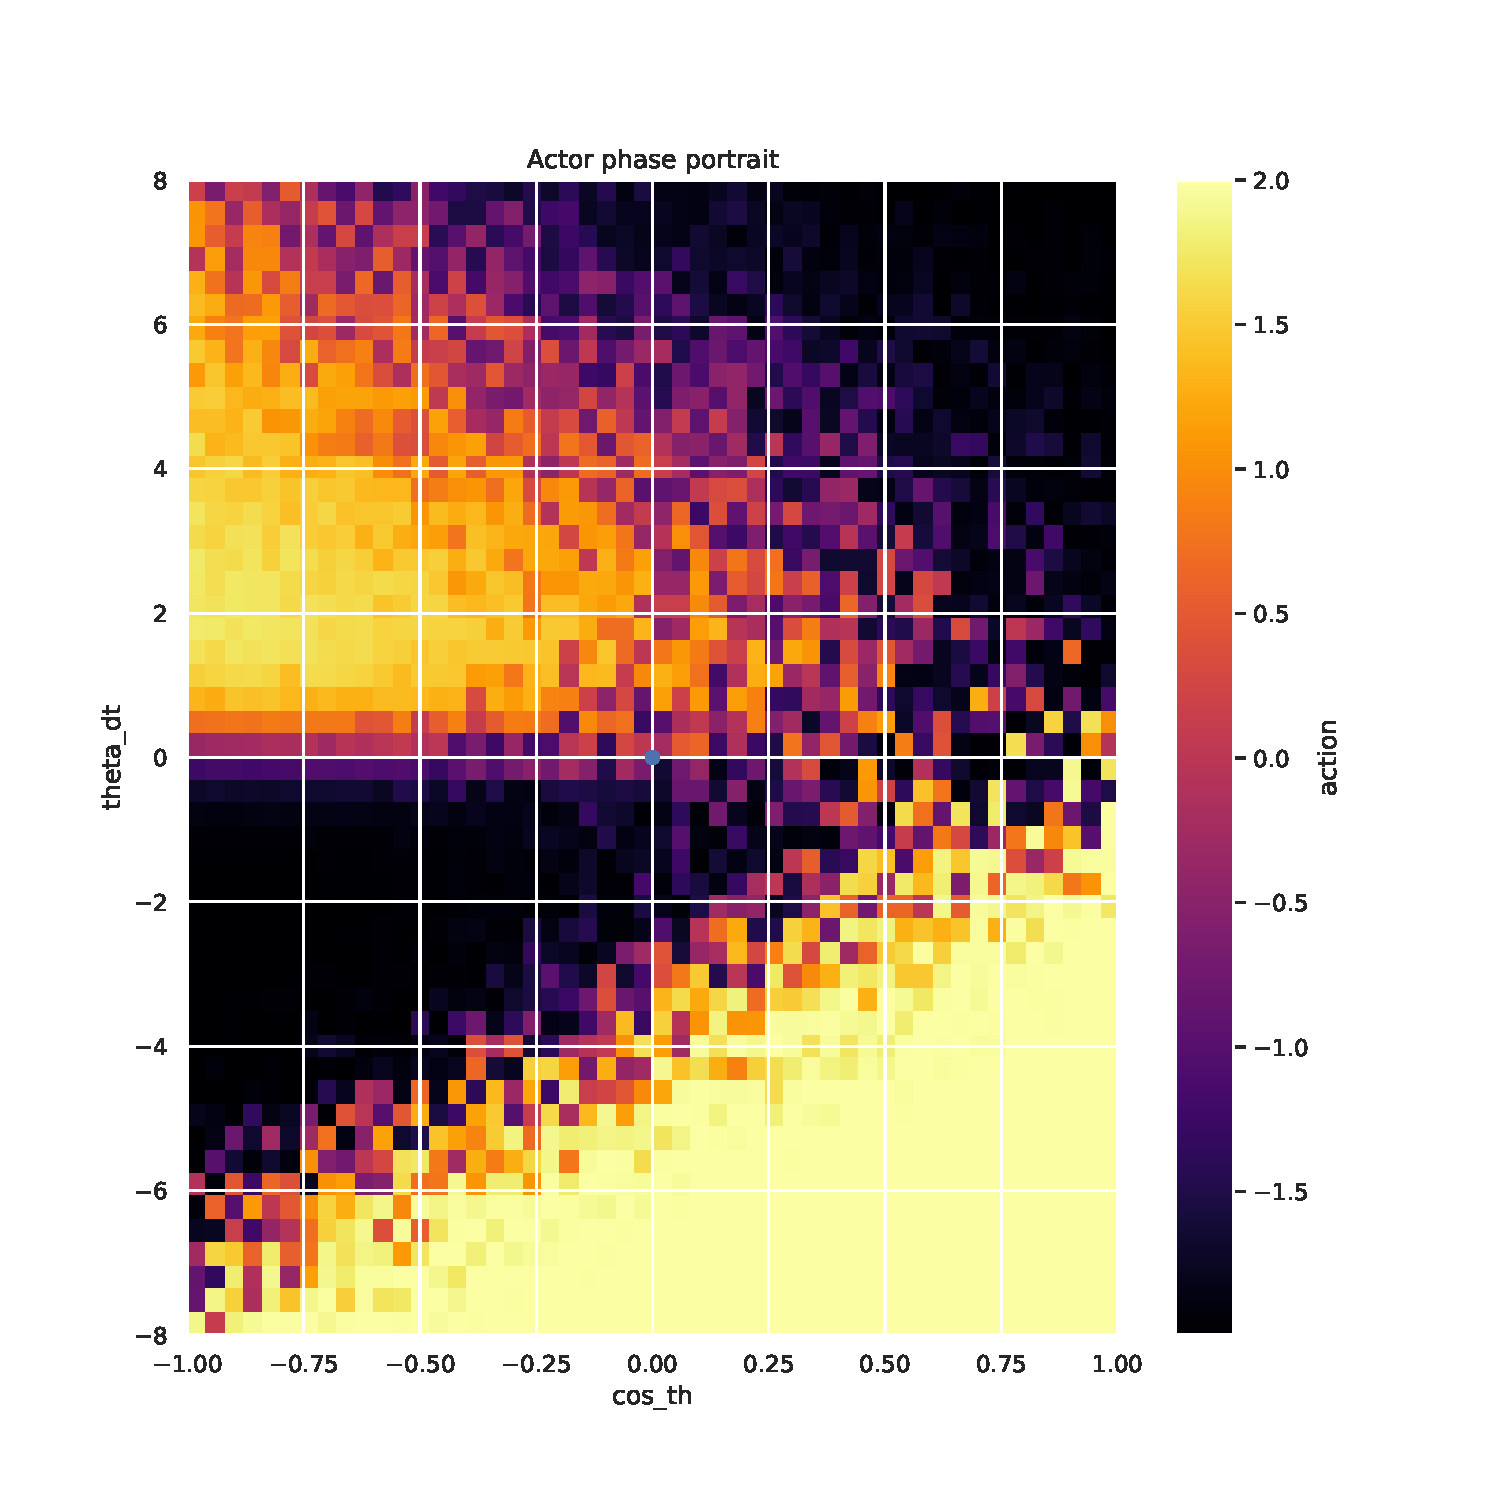
\includegraphics[width=\textwidth]{figures/sac_itr2/8_actor_SAC__post_Pendulum-v0.pdf}
        \caption{Acteur entraîné}
    \end{subfigure}
    \begin{subfigure}{0.45\textwidth}
        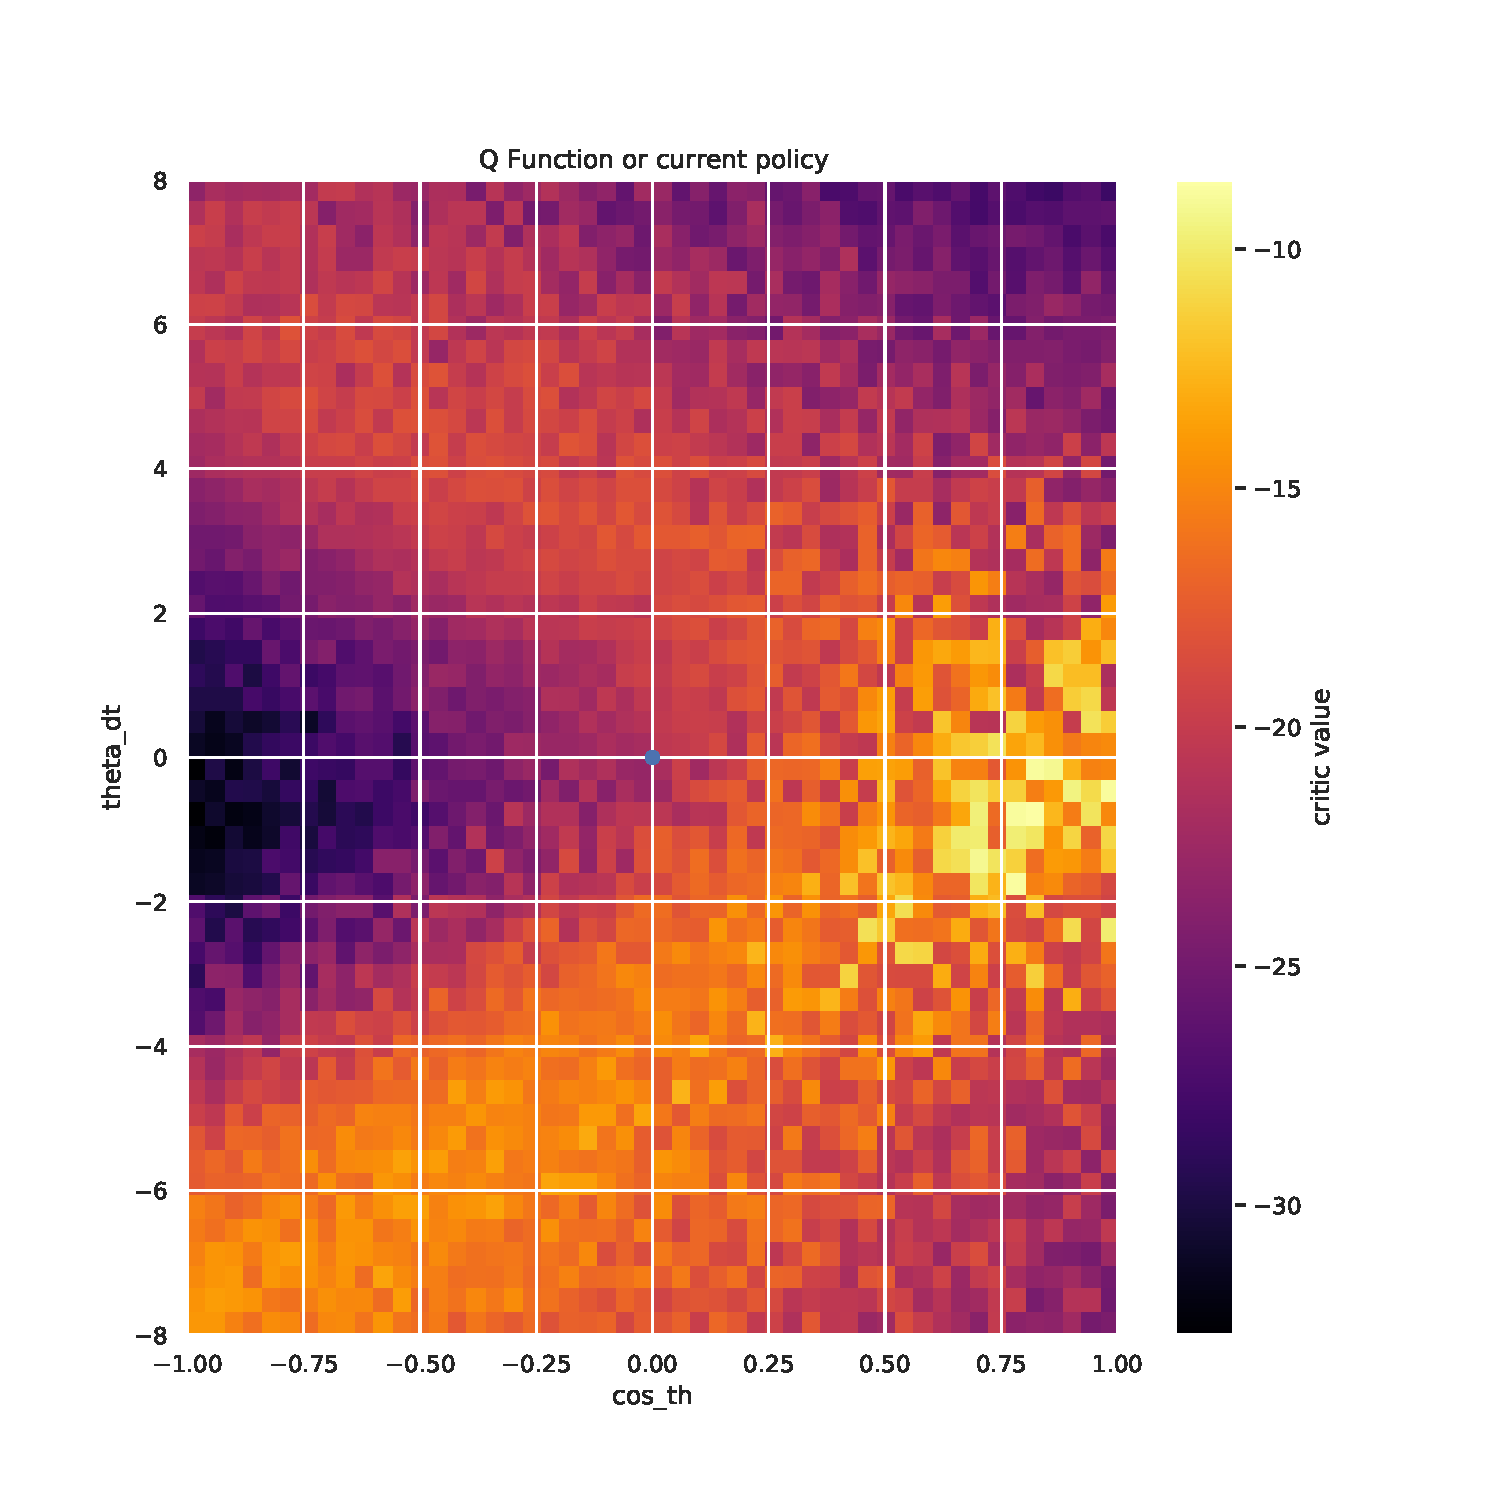
\includegraphics[width=\textwidth]{figures/sac_itr2/8_critic_SAC_q1_post_Pendulum-v0.pdf}
        \caption{Critique entraînée}
    \end{subfigure}
    \caption{Valeurs de l'acteur et de la critique avec l'algorithme SAC dans un cas où l'apprentissage n'est pas fructueux}
    \label{fig:sac:itr2}
\end{figure}

Avec le ratio d'apprentissage de \(\alpha\) à $0.02$, l'ensemble des résultats obtenus sont cohérents et quasi similaires. Certaines itérations présentent encore une faible exploration d'un coté du pendule. Mais nous n'observons pas de cas critique comme sur la figure~\ref{fig:sac:preli_failed}. En effet, la forme de la politique désirée ressemble à un \(>\) de couleur clair. Si le \(\cos(\theta) = -1\) le pendule est en bas et ne doit pas être à une vitesse faible (une zone sombre). Si le \(\cos(\theta) = 1\), alors le pendule est en haut et doit alors rester immobile. Cet état est à favoriser pour maximiser la récompense (zone claire).